\documentclass[11pt,a4paper]{article}
\usepackage[margin=2.3cm]{geometry}
\usepackage{amsmath,amssymb,bm}
\usepackage{siunitx}
\usepackage{booktabs}
\usepackage{nicefrac}
\usepackage{graphicx}
\usepackage{tikz}
\usetikzlibrary{arrows.meta,calc,positioning,patterns}
\usepackage{pgfplots}
\pgfplotsset{compat=1.17}
\usepackage{enumitem}
\usepackage{float}
\tikzset{capt/.style={text width=5.2cm,align=center}}
\usepackage[colorlinks=true,linkcolor=blue!60!black,urlcolor=blue!60!black]{hyperref}
\usepackage{fancyhdr}
\usepackage{tcolorbox}
\tcbuselibrary{skins,breakable}
\sisetup{per-mode=symbol,detect-all}

\newtcolorbox{keybox}[1]{title={#1},colback=blue!4,colframe=blue!50!black,fonttitle=\bfseries,breakable}
\newtcolorbox{examplebox}[1]{title={#1},colback=green!4,colframe=green!40!black,fonttitle=\bfseries,breakable}
\newtcolorbox{aerobox}[1]{title={#1},colback=orange!5,colframe=orange!60!black,fonttitle=\bfseries,breakable}

\pagestyle{fancy}
\fancyhf{}
\lhead{
\includegraphics[height=0.6cm]{logos/itu_logo_laci.pdf}\ \ UCK 364E Design of Machine Elements}
\setlength{\headheight}{20pt}
\rhead{Lecture 8 -- Notes}
\cfoot{\thepage}

% small pictograms of weld-group patterns for the property table
\newcommand{\wic}[1]{\raisebox{-3.2mm}{\begin{tikzpicture}[scale=0.36,line cap=round]\draw[black!35,line width=0.3pt] (-1,-1) rectangle (1,1);#1\end{tikzpicture}}}

\title{\textbf{UCK 364E Design of Machine Elements}\\[4pt]
\Large Lecture 8: Welds in Bending and Torsion, and Adhesive Bonding\\[2pt]
\large The weld as a line --- and the joint with no fastener and no heat}
\author{Prof.\ Dr.\ Onur Tunçer\\ Department of Aeronautical Engineering, Istanbul Technical University}
\date{Fall 2026}

\begin{document}
\maketitle

\section*{Learning objectives}
By the end of this lecture you should be able to:
\begin{enumerate}[nosep]
  \item Recognise whether a weld group is loaded in torsion, in bending, or both.
  \item Treat a weld group as a line: find its centroid and its unit second moments $I_u$ and $J_u$.
  \item Find the critical point of a weld group in torsion and the resultant throat stress there.
  \item Find the throat stress in a weld group in bending, and compare arrangements of the same
        weld length.
  \item Size the weld around a tube carrying axial load, bending and torsion together, working in
        force per unit length.
  \item Name the four ways an adhesive joint can be loaded and say which to design for.
  \item Explain why the shear stress in a bonded lap peaks at its ends, estimate the peak, and
        explain why a longer overlap does not make a stronger joint.
  \item Rank the common bonded joint configurations and say what each improvement buys.
  \item Say why bonding, like welding, is a special process --- and what happened at Aloha when
        the bond was not there.
\end{enumerate}

\section{Why this lecture exists}

Lecture 7 treated a weld carrying a force along or across its own length: divide by the throat
area. Real welded parts are rarely that kind. A bracket hangs a load out from a column. A tube is
welded to a fitting and is bent and twisted. The weld then carries a \emph{moment}, and a moment is
not shared equally along a weld any more than it was shared equally among the bolts of Lecture 6.

\medskip
The method is the one you already know from the bolt group: a direct part, a part from the moment
that grows with distance from the centroid, added as vectors at the worst point. The only new idea
is that the ``fasteners'' are now continuous, so sums become integrals --- and somebody has already
done the integrals.

\medskip
The second half of the lecture is the last of the permanent joints: the adhesive bond. It has no
hole, no heat-affected zone and no toe. It spreads the load over an area instead of concentrating
it at points. It also has a habit of carrying nearly all of that load at its two ends, and it is
the only joint in this course whose strength cannot be inspected at all once it is made.

\begin{figure}[H]\centering
\resizebox{\textwidth}{!}{% Three ways a weld group is loaded by a moment.
\begin{tikzpicture}[>=Latex,line join=round]
\tikzset{pl/.style={fill=black!10,draw=black,line width=0.6pt}, col/.style={fill=black!25,draw=black,line width=0.6pt},
  wd/.style={line width=2.6pt,line cap=round}, ld/.style={->,line width=1.2pt}, ttl/.style={font=\normalsize\bfseries,anchor=north,align=center},
  sub/.style={font=\small,anchor=north,align=center,text=black!65}}
% (a) in-plane: torsion
\begin{scope}
 \path[col] (-0.9,-1.7) rectangle (0.9,1.7);
 \path[pl] (-0.5,-0.9) rectangle (3.2,0.9);
 \draw[wd] (0.9,0.9) -- (-0.5,0.9) -- (-0.5,-0.9) -- (0.9,-0.9);
 \draw[ld] (2.9,1.6) -- (2.9,0.95); \node[font=\normalsize,anchor=south] at (2.9,1.6) {$P$};
 \draw[->,line width=0.5pt] (0.75,0) arc[start angle=0,end angle=-250,radius=0.45];
 \node[ttl] at (1.1,-1.95) {(a) In-plane load};
 \node[sub] at (1.1,-2.4) {the group is \textbf{twisted}: torsion};
\end{scope}
% (b) out-of-plane: bending
\begin{scope}[xshift=6.3cm]
 \path[col] (-0.9,-1.7) rectangle (-0.3,1.7);
 \path[pl] (-0.3,-0.75) rectangle (3.0,0.75);
 \draw[wd] (-0.3,0.75) -- (-0.3,-0.75);
 \draw[ld] (2.7,1.5) -- (2.7,0.8); \node[font=\normalsize,anchor=south] at (2.7,1.5) {$P$};
 \draw[->,line width=0.5pt] (-0.3,1.05) -- (0.25,1.05); \draw[->,line width=0.5pt] (0.25,-1.05) -- (-0.3,-1.05);
 \node[ttl] at (1.0,-1.95) {(b) Out-of-plane load};
 \node[sub] at (1.0,-2.4) {the group is \textbf{bent}};
\end{scope}
% (c) tube
\begin{scope}[xshift=12.4cm]
 \path[col] (-0.9,-1.7) rectangle (-0.3,1.7);
 \path[pl] (-0.3,-0.45) rectangle (3.0,0.45);
 \draw[wd] (-0.3,0.45) -- (-0.3,-0.45);
 \draw[line width=0.4pt,dash pattern=on 6pt off 2pt on 1pt off 2pt] (-1.1,0) -- (3.5,0);
 \draw[ld] (2.7,1.3) -- (2.7,0.5); \node[font=\normalsize,anchor=south] at (2.7,1.3) {$P$};
 \draw[->,line width=0.9pt] (3.25,-0.42) arc[start angle=-70,end angle=70,x radius=0.22,y radius=0.45]; \node[font=\normalsize,anchor=west] at (3.5,0) {$T$};
 \node[ttl] at (1.1,-1.95) {(c) Tube welded all round};
 \node[sub] at (1.1,-2.4) {bending \emph{and} torsion};
\end{scope}
\end{tikzpicture}
}
\caption{Three ways a weld group meets a moment. In (a) the moment vector is normal to the plane
of the welds; in (b) it lies in that plane.}
\label{fig:cases}
\end{figure}

\section{The weld as a line}
\label{sec:line}

A fillet weld is long and thin. Its throat $a=0.707h$ is small compared with its length, so for
the purpose of finding areas and second moments it can be treated as a \textbf{line} with a
uniform width $a$. Every property of the weld group is then the property of a line, times the
throat:
\begin{equation}
A = a\,L,\qquad I = a\,I_u,\qquad J = a\,J_u,\qquad a=0.707\,h .
\label{eq:unit}
\end{equation}
$L$ is the total length of weld, and $I_u$ and $J_u$ are the \emph{unit} second moments of area
--- of a line of unit width --- about the centroid of the group. They have units of length cubed.

\begin{center}\small
\renewcommand{\arraystretch}{1.9}
\begin{tabular}{@{}clll@{}}
\toprule
\textbf{Pattern} & \textbf{Length $L$} & \textbf{Bending, $I_u$ about the horizontal axis} & \textbf{Torsion, $J_u$}\\
\midrule
\wic{\draw[line width=1.6pt] (0,-1) -- (0,1);} & $d$ & $\dfrac{d^3}{12}$ & $\dfrac{d^3}{12}$\\
\wic{\draw[line width=1.6pt] (-1,-1) -- (-1,1) (1,-1) -- (1,1);} & $2d$ & $\dfrac{d^3}{6}$ & $\dfrac{d\,(3b^2+d^2)}{6}$\\
\wic{\draw[line width=1.6pt] (-1,1) -- (1,1) (-1,-1) -- (1,-1);} & $2b$ & $\dfrac{b\,d^2}{2}$ & $\dfrac{b\,(3d^2+b^2)}{6}$\\
\wic{\draw[line width=1.6pt] (1,1) -- (-1,1) -- (-1,-1) -- (1,-1);} & $2b+d$ & $\dfrac{d^2\,(6b+d)}{12}$ &
  $\dfrac{8b^3+6bd^2+d^3}{12}-\dfrac{b^4}{2b+d}$\\
\wic{\draw[line width=1.6pt] (-1,-1) rectangle (1,1);} & $2(b+d)$ & $\dfrac{d^2\,(3b+d)}{6}$ & $\dfrac{(b+d)^3}{6}$\\
\wic{\draw[line width=1.6pt] (0,0) circle (1);} & $2\pi r$ & $\pi r^3$ & $2\pi r^3$\\
\bottomrule
\end{tabular}
\end{center}

\noindent In every row $b$ is the horizontal dimension of the pattern and $d$ the vertical one. For
the three-sided pattern the centroid lies $\bar x=b^2/(2b+d)$ from the closed side. These are the
entries of Shigley's Tables 9--1 and 9--2. You can always check one: $J_u=I_{u,x}+I_{u,y}$.

\begin{keybox}{Why this is worth doing}
The unit properties depend only on the \emph{layout} of the weld, not on its size. So you can
choose where to put the weld before you know how big it has to be --- and, as Example 8.2 will
show, where you put it matters more than how much of it there is.
\end{keybox}

\section{Weld groups in torsion}
\label{sec:torsion}

When the load lies in the plane of the welds but does not pass through their centroid
(figure~\ref{fig:cases}a), move it to the centroid. It becomes a force $V$ through the centroid and
a moment $M=Ve$ about it.

\begin{enumerate}[leftmargin=*,itemsep=2pt]
\item \textbf{Primary shear}, the same everywhere, in the direction of the load:
  \[ \tau'=\frac{V}{A}. \]
\item \textbf{Secondary shear}, perpendicular to the radius from the centroid and proportional to it:
  \[ \tau''=\frac{M\,r}{J}. \]
\item \textbf{Add as vectors} at the point where the two combine worst --- usually the point
  furthest from the centroid on the side nearest the load.
\end{enumerate}

This is the bolt group of Lecture 6 word for word, with $A$ in place of $n$ and $J$ in place of
$\sum r^2$.

\begin{figure}[H]\centering
\resizebox{0.72\textwidth}{!}{% Example 8.1: a C-shaped weld group in torsion. 1 mm = 0.035 cm.
\begin{tikzpicture}[>=Latex,line join=round]
\tikzset{lb/.style={font=\footnotesize}, sm/.style={font=\scriptsize}, dimn/.style={<->,line width=0.4pt}, ext/.style={line width=0.25pt}}
\def\g{0.035}
\fill[black!22] (-1.6,-3.2) rectangle (3.3,3.2); \draw[line width=0.6pt] (-1.6,-3.2) rectangle (3.3,3.2);
\fill[black!8] (0,-60*\g) rectangle (270*\g,60*\g); \draw[line width=0.6pt] (0,-60*\g) rectangle (270*\g,60*\g);
\draw[line width=2.8pt,line cap=round] (80*\g,60*\g) -- (0,60*\g) -- (0,-60*\g) -- (80*\g,-60*\g);
% centroid
\def\xb{22.86}
\draw[line width=0.3pt] (\xb*\g-0.25,0) -- (\xb*\g+0.25,0) (\xb*\g,-0.25) -- (\xb*\g,0.25); \fill (\xb*\g,0) circle (1.4pt);
\node[sm,anchor=north west] at (\xb*\g+0.02,-0.04) {G};
% load
\draw[->,line width=1.5pt] (250*\g,3.4) -- (250*\g,2.2); \node[lb,anchor=south] at (250*\g,3.4) {$P=\SI{20}{kN}$};
% radius to A
\draw[line width=0.5pt,dashed] (\xb*\g,0) -- (80*\g,60*\g); \node[sm,anchor=south east] at (52*\g,31*\g) {$r$};
\fill (80*\g,60*\g) circle (1.8pt); \node[lb,anchor=south] at (80*\g,60*\g+0.08) {A};
% vectors at A : tau' down, tau'' perpendicular to r (clockwise): direction (y,-x)/r = (60,-57.14)/82.86
\def\f{0.024}
\draw[->,line width=1.0pt] (80*\g,60*\g) -- ++(0,-16.84*\f);
\draw[->,line width=1.0pt] (80*\g,60*\g) -- ++(70.2*\f,-66.9*\f);
\draw[->,line width=1.6pt] (80*\g,60*\g) -- ++(70.2*\f,-83.7*\f);
\node[sm,anchor=east] at (80*\g-0.05,60*\g-0.3) {$\tau'$};
\node[sm,anchor=south west] at (80*\g+70.2*\f,60*\g-66.9*\f+0.02) {$\tau''$};
\node[sm,anchor=north west] at (80*\g+70.2*\f,60*\g-83.7*\f-0.02) {$\tau$};
% dimensions
\draw[ext] (0,-60*\g-0.1) -- (0,-3.75) (80*\g,-60*\g-0.15) -- (80*\g,-3.75) (250*\g,-60*\g-0.1) -- (250*\g,-4.35) (0,-3.75) -- (0,-4.35);
\draw[dimn] (0,-3.55) -- (80*\g,-3.55); \node[sm,anchor=north] at (40*\g,-3.57) {80};
\draw[dimn] (0,-4.15) -- (250*\g,-4.15); \node[sm,anchor=north] at (125*\g,-4.17) {250};
\draw[ext] (-0.1,60*\g) -- (-2.25,60*\g) (-0.1,-60*\g) -- (-2.25,-60*\g); \draw[dimn] (-2.05,-60*\g) -- (-2.05,60*\g); \node[sm,anchor=east] at (-2.1,0) {120};
\node[sm,anchor=west] at (3.45,-2.8) {column};
\node[sm] at (6.3,0) {plate};
\end{tikzpicture}
}
\caption{Example 8.1. The three-sided weld group, its centroid G, and the stresses at the critical
point A.}
\label{fig:torsion}
\end{figure}

\begin{examplebox}{Example 8.1 --- a bracket plate welded on three sides}
A plate is lap-welded to a column by a three-sided fillet, $h=\SI{6}{mm}$: a vertical run of
$d=\SI{120}{mm}$ and two horizontal runs of $b=\SI{80}{mm}$. A load $P=\SI{20}{kN}$ acts downward
\SI{250}{mm} from the vertical run. Find the largest throat stress. E70xx electrode.

\medskip
\textbf{Group properties.} $L=2(80)+120=\SI{280}{mm}$; \ $A=0.707(6)(280)=\SI{1188}{mm^2}$.
\[ \bar x=\frac{80^2}{2(80)+120}=\SI{22.9}{mm},\qquad
   J_u=\frac{8(80)^3+6(80)(120)^2+120^3}{12}-\frac{80^4}{280}=\SI{915000}{mm^3} \]
\[ J=0.707(6)(915\,000)=\SI{3.88e6}{mm^4} \]

\textbf{Loads at the centroid.} $e=250-22.9=\SI{227.1}{mm}$; \ $M=20\,000\times227.1=\SI{4.54e6}{N.mm}$.

\textbf{Critical point A}, the tip of the upper run: $x=80-22.9=\SI{57.1}{mm}$, $y=\SI{60}{mm}$,
$r=\SI{82.9}{mm}$.
\[ \tau'=\frac{20\,000}{1188}=\SI{16.8}{MPa}\ \text{(down)} \]
\[ \tau''_x=\frac{M\,y}{J}=\frac{4.54\times10^{6}(60)}{3.88\times10^{6}}=\SI{70.2}{MPa} \]
\[ \tau''_y=\frac{M\,x}{J}=\frac{4.54\times10^{6}(57.1)}{3.88\times10^{6}}=\SI{66.9}{MPa}\ \text{(down)} \]
\[ \tau=\sqrt{70.2^2+(66.9+16.8)^2}=\mathbf{\SI{109}{MPa}} \]

Against $\tau_{\text{all}}=0.30\times482=\SI{145}{MPa}$ the factor is 1.33.

\medskip
\textbf{Read the numbers.} The moment contributes \SI{97}{MPa} and the direct shear 17. A designer
who divided the load by the throat area would have reported \SI{17}{MPa} and a factor of 8.6. At
the other end of the same weld, the corner on the closed side, the stress is \SI{71}{MPa}: the weld
is far from uniformly used.
\end{examplebox}

\section{Weld groups in bending}
\label{sec:bending}

When the load is out of the plane of the welds (figure~\ref{fig:cases}b), the moment tries to peel
one edge of the group off and push the other on. The stress from the moment is now \emph{normal}
to the weld line, and it varies linearly with distance from the neutral axis of the group:
\begin{equation}
\tau'=\frac{V}{A},\qquad \tau''=\frac{M\,c}{I},\qquad \tau=\sqrt{\tau'^2+\tau''^2}.
\end{equation}
Two conventions are hiding in that line, and both come from Lecture 7. The bending stress acts
across the throat as a mixture of normal and shear stress, but it is \emph{treated as a shear on
the throat} --- the same safe simplification as before. And because the direct shear lies along
the joint face while the bending stress is normal to it, the two are at right angles and add as
the root of the sum of squares.

\begin{figure}[H]\centering
\resizebox{\textwidth}{!}{% Example 8.2: the same weld length arranged three ways, seen looking along the bracket.
\begin{tikzpicture}[>=Latex,line join=round]
\tikzset{lb/.style={font=\normalsize}, sm/.style={font=\small}, wd/.style={line width=2.8pt,line cap=round}, sec/.style={fill=black!10,draw=black,line width=0.5pt}}
% side view
\begin{scope}
 \fill[black!25] (-0.7,-1.9) rectangle (0,1.9); \draw[line width=0.6pt] (-0.7,-1.9) rectangle (0,1.9);
 \fill[black!10] (0,-1.0) rectangle (3.4,1.0); \draw[line width=0.6pt] (0,-1.0) rectangle (3.4,1.0);
 \draw[wd] (0,1.0) -- (0,-1.0);
 \draw[->,line width=1.4pt] (3.0,1.9) -- (3.0,1.05); \node[lb,anchor=south] at (3.0,1.9) {$P=\SI{8}{kN}$};
 \draw[<->,line width=0.4pt] (0,-1.4) -- (3.0,-1.4); \node[sm,anchor=north] at (1.5,-1.42) {150};
 \draw[<->,line width=0.4pt] (3.7,-1.0) -- (3.7,1.0); \node[sm,anchor=west] at (3.75,0) {100};
 \node[lb,anchor=north] at (1.4,-2.2) {side view};
\end{scope}
% three weld patterns, end view
\foreach \xo/\ttl/\iu/\tv in {7.0/{two vertical}/{$d^3/6$}/85, 10.6/{two horizontal}/{$bd^2/2$}/30, 14.2/{all round}/{$d^2(3b+d)/6$}/22}{
 \begin{scope}[xshift=\xo cm]
  \path[sec] (-1.0,-1.0) rectangle (1.0,1.0);
  \draw[line width=0.3pt,dash pattern=on 5pt off 2pt on 1pt off 2pt] (-1.5,0) -- (1.5,0);
  \node[lb,anchor=north] at (0,-1.3) {\ttl};
  \node[sm,anchor=north] at (0,-1.95) {$I_u=$ \iu};
  \node[lb,anchor=north] at (0,-2.65) {$\tau=\SI{\tv}{MPa}$};
 \end{scope}}
\begin{scope}[xshift=7.0cm] \draw[wd] (-1.0,-1.0) -- (-1.0,1.0) (1.0,-1.0) -- (1.0,1.0); \end{scope}
\begin{scope}[xshift=10.6cm] \draw[wd] (-1.0,1.0) -- (1.0,1.0) (-1.0,-1.0) -- (1.0,-1.0); \end{scope}
\begin{scope}[xshift=14.2cm] \draw[wd] (-1.0,-1.0) rectangle (1.0,1.0); \end{scope}
\node[sm,anchor=west] at (15.75,0) {neutral axis};
\end{tikzpicture}
}
\caption{Example 8.2. The same bracket, and three ways to weld a $100\times\SI{100}{mm}$ end to the
column.}
\label{fig:bending}
\end{figure}

\begin{examplebox}{Example 8.2 --- where the weld is matters more than how much there is}
A bracket with a $100\times\SI{100}{mm}$ end is welded to a column and carries $P=\SI{8}{kN}$ at
\SI{150}{mm}. Fillets $h=\SI{6}{mm}$. $M=8000\times150=\SI{1.2e6}{N.mm}$, $c=\SI{50}{mm}$.

\medskip
\textbf{(a) Two vertical welds, $d=100$.} $A=1.414(6)(100)=\SI{848}{mm^2}$;
$I_u=100^3/6=\SI{166700}{mm^3}$; $I=0.707(6)(166\,700)=\SI{7.07e5}{mm^4}$.
\[ \tau'=\frac{8000}{848}=\SI{9.4}{MPa},\qquad \tau''=\frac{1.2\times10^{6}(50)}{7.07\times10^{5}}=\SI{84.9}{MPa},\qquad \tau=\mathbf{\SI{85}{MPa}} \]

\textbf{(b) Two horizontal welds, $b=100$, \SI{100}{mm} apart.} The same \SI{200}{mm} of weld.
$I_u=bd^2/2=\SI{500000}{mm^3}$, three times as much:
\[ \tau''=\SI{28.3}{MPa},\qquad \tau=\mathbf{\SI{30}{MPa}} \]

\textbf{(c) Welded all round.} Twice the weld. $I_u=d^2(3b+d)/6=\SI{666700}{mm^3}$:
\[ \tau'=\SI{4.7}{MPa},\qquad \tau''=\SI{21.2}{MPa},\qquad \tau=\mathbf{\SI{22}{MPa}} \]

\medskip
Moving the same weld from the sides to the top and bottom cut the stress by a factor of 2.9.
Doubling the weld after that gained another 1.4. \textbf{Weld metal far from the neutral axis does
the work in bending} --- exactly as flange material does in a beam.

\medskip
\emph{And the catch,} from Lecture 7: the top weld of (b) is a transverse weld across the most
highly stressed fibre of the bracket. Statically it is the right answer. If the load cycles, that
weld toe is where the crack starts, and the arrangement must be checked as a fatigue detail.
\end{examplebox}

\section{A tube welded all round: working in force per unit length}
\label{sec:tube}

For design the unit properties are used the other way round. You do not know the weld size yet, so
divide the loads by the \emph{line} properties and get a force per unit length of weld, $f$, in
N/mm. The throat needed is then simply
\begin{equation}
a=\frac{f}{\tau_{\text{all}}},\qquad h=\frac{a}{0.707}.
\end{equation}
For a ring of weld of radius $r$, the table gives $L=2\pi r$, $I_u=\pi r^3$, $J_u=2\pi r^3$, so
\begin{equation}
f_N=\frac{N}{2\pi r},\qquad f_M=\frac{M\,r}{\pi r^3}=\frac{M}{\pi r^2},\qquad
f_T=\frac{T\,r}{2\pi r^3}=\frac{T}{2\pi r^2}.
\label{eq:ring}
\end{equation}
$f_N$ and $f_M$ both act along the tube axis and add directly at the extreme fibre; $f_T$ acts
around the circumference, at right angles to them.

\begin{examplebox}{Example 8.3 --- the end weld of an engine-mount tube}
A $25.4\times\SI{0.889}{mm}$ 4130N tube is fillet-welded all round to an end fitting. At limit load
the weld carries an axial tension $N=\SI{12}{kN}$, a bending moment $M=\SI{40}{N.m}$ and a torque
$T=\SI{30}{N.m}$. The weld metal is allowed $F_{su}=\SI{300}{MPa}$ in shear at ultimate. Size the
weld, and check the tube beside it.

\medskip
\textbf{Line loads,} $r=\SI{12.7}{mm}$:
\[ f_N=\frac{12\,000}{2\pi(12.7)}=\SI{150}{N/mm},\qquad f_M=\frac{40\,000}{\pi(12.7)^2}=\SI{79}{N/mm} \]
\[ f_T=\frac{30\,000}{2\pi(12.7)^2}=\SI{30}{N/mm} \]
\[ f=\sqrt{(150+79)^2+30^2}=\SI{231}{N/mm}\ \text{at limit};\qquad f_u=1.5\times231=\SI{347}{N/mm} \]

\textbf{Weld size.} $a=347/300=\SI{1.16}{mm}$, so $h=1.16/0.707=\mathbf{\SI{1.6}{mm}}$ --- a leg of
about 1.8 times the wall. Call up \textbf{a1.2} all round.

\medskip
\textbf{The tube beside the weld.} $A=\SI{68.5}{mm^2}$; $Z\approx\pi r_m^2 t=\pi(12.26)^2(0.889)=
\SI{419}{mm^3}$.
\[ \sigma=\frac{12\,000}{68.5}+\frac{40\,000}{419}=175+95=\SI{271}{MPa}\ \text{at limit};\qquad \SI{406}{MPa}\ \text{at ultimate} \]
Against the welded allowable of Lecture 7, \SI{552}{MPa} for a square-cut end:
$\mathrm{MS}=552/406-1=\mathbf{+0.36}$.

\medskip
Two margins, two different materials: the weld metal on its throat, and the heat-affected tube on
its wall. Project 1 needs both at every cluster.
\end{examplebox}

\subsection*{If the load cycles}

Nothing in this lecture changes the fatigue rules of Lecture 7; it only tells you where on the
group to apply them. Find the stress \emph{range} at the critical point --- point A in Example 8.1,
the extreme fibre in Examples 8.2 and 8.3 --- and use the detail category that fits: a
load-carrying fillet is checked at its root on the throat stress, and the member beside it at the
weld toe. Remember where Shigley's worst factor was: the \emph{end of a parallel fillet}. In
Example 8.1 that is exactly point A.

\section{Adhesive bonding}
\label{sec:bond}

\subsection{What a bond offers, and what it asks}

\begin{keybox}{What a bonded joint trades}
\textbf{In its favour.} No holes, so no net-section loss and no stress concentration at a
fastener. The load is spread over an area. It seals. It joins thin sheet that could not take a
rivet, and dissimilar materials that could not be welded. A well-made bonded joint has a much
better fatigue life than a riveted one in the same sheet.

\medskip
\textbf{Against it.} Its strength depends on a surface preparation you cannot see afterwards. It is
weak in peel. It is sensitive to moisture and temperature, and it creeps. It cannot be taken
apart. And \textbf{no inspection can measure the strength of a finished bond}: ultrasound finds a
gap, but two surfaces in contact with no adhesion look sound.
\end{keybox}

\begin{aerobox}{Where you meet it}
Honeycomb sandwich panels --- floors, control surfaces, fairings --- are bonded by definition: the
face sheets are held to the core by adhesive and nothing else. Stringers have been bonded to skins
since the wooden de Havilland aircraft of the 1940s and the metal Fokker F27 of the 1950s. Every
composite structure is a bonded structure. And the threadlocker of Lecture 5 is an adhesive: an
anaerobic one, which cures when it is shut away from air between metal surfaces.
\end{aerobox}

\subsection{Four ways to load an adhesive}

\begin{figure}[H]\centering
\resizebox{\textwidth}{!}{% The four ways to load an adhesive joint.
\begin{tikzpicture}[>=Latex,line join=round]
\tikzset{ad/.style={fill=black!12,draw=black,line width=0.6pt}, gl/.style={fill=black!60}, ld/.style={->,line width=1.2pt},
  ttl/.style={font=\normalsize\bfseries,anchor=north}, sub/.style={font=\small,anchor=north,text=black!65,align=center}}
% shear
\begin{scope}
 \path[ad] (-1.9,0.06) rectangle (0.7,0.42); \path[ad] (-0.7,-0.42) rectangle (1.9,-0.06); \path[gl] (-0.7,-0.06) rectangle (0.7,0.06);
 \draw[ld] (-1.95,0.24) -- (-2.6,0.24); \draw[ld] (1.95,-0.24) -- (2.6,-0.24);
 \node[ttl] at (0,-1.75) {Shear}; \node[sub] at (0,-2.2) {the whole area works\\ \textbf{design for this}};
\end{scope}
% tension
\begin{scope}[xshift=5.3cm]
 \path[ad] (-0.9,0.06) rectangle (0.9,0.9); \path[ad] (-0.9,-0.9) rectangle (0.9,-0.06); \path[gl] (-0.9,-0.06) rectangle (0.9,0.06);
 \draw[ld] (0,0.95) -- (0,1.55); \draw[ld] (0,-0.95) -- (0,-1.55);
 \node[ttl] at (0,-1.75) {Tension}; \node[sub] at (0,-2.2) {acceptable if truly uniform ---\\ it rarely is};
\end{scope}
% cleavage
\begin{scope}[xshift=10.2cm]
 \path[ad] (-1.2,0.06) rectangle (1.2,0.7); \path[ad] (-1.2,-0.7) rectangle (1.2,-0.06); \path[gl] (-1.2,-0.06) rectangle (1.2,0.06);
 \draw[ld] (-1.0,0.75) -- (-1.0,1.4); \draw[ld] (-1.0,-0.75) -- (-1.0,-1.4);
 \node[ttl] at (0,-1.75) {Cleavage}; \node[sub] at (0,-2.2) {one edge carries it all\\ \textbf{avoid}};
\end{scope}
% peel
\begin{scope}[xshift=15.0cm]
 \path[ad] (-1.4,-0.6) rectangle (1.4,-0.06); \path[gl] (-0.3,-0.06) rectangle (1.4,0.04);
 \draw[line width=3pt,black!45,line cap=butt] (1.4,0.09) -- (-0.3,0.09) .. controls (-0.75,0.12) and (-0.95,0.5) .. (-1.0,1.15);
 \draw[ld] (-1.0,1.2) -- (-1.0,1.8);
 \node[ttl] at (0,-1.75) {Peel}; \node[sub] at (0,-2.2) {a line carries it all\\ \textbf{avoid}};
\end{scope}
\end{tikzpicture}
}
\caption{Adhesives are strong when the whole bond area shares the load, and weak when the load
concentrates on a line.}
\label{fig:modes}
\end{figure}

The whole art of bonded joint design is in this figure: \textbf{arrange the joint so the adhesive
is in shear, and keep peel and cleavage out}. A structural adhesive that carries
\SI{30}{MPa} in shear over an area may carry only a few newtons per millimetre of width in peel.

\subsection{Adhesives}

\begin{center}\footnotesize
\begin{tabular}{@{}p{3.5cm}p{2.6cm}p{2.5cm}p{6.2cm}@{}}
\toprule
\textbf{Family} & \textbf{Lap shear, MPa} & \textbf{Service limit} & \textbf{Where you meet it}\\
\midrule
Epoxy film, hot cured & 25--40 & 120--\SI{175}{\degree C} & primary structural bonds, honeycomb\\
Epoxy paste, two-part & 15--30 & about \SI{80}{\degree C} & repairs, fittings, shimming\\
Toughened acrylic & 15--25 & about \SI{100}{\degree C} & fast assembly, less surface preparation\\
Anaerobic & 10--25 & about \SI{150}{\degree C} & threadlocking, retaining bearings and bushes\\
Cyanoacrylate & 10--20 & about \SI{80}{\degree C} & small parts; brittle, poor in peel\\
Polyurethane, silicone & 1--15 & to \SI{200}{\degree C} (silicone) & sealing, flexible joints, windscreens\\
\bottomrule
\end{tabular}
\end{center}

\noindent These are indicative room-temperature figures for comparison only. The number you design
with comes from the adhesive's data sheet, for your adherends, your surface preparation and your
temperature --- and it is far lower hot and wet than it is in the brochure.

\subsection{The lap joint: where the load actually goes}
\label{sec:lap}

The obvious calculation for a lap joint of width $b$ and overlap $l$ is the average shear stress,
\begin{equation}
\tau_{\text{avg}}=\frac{P}{b\,l},
\end{equation}
and it is as misleading as dividing a row of fasteners equally. The reason is the one you met in
Lecture 6. At one end of the overlap, one sheet carries all of the load and the other carries
none; they stretch by different amounts; the adhesive between them is sheared hard. In the middle
both sheets carry half, they stretch alike, and the adhesive has almost nothing to do.

\medskip
For two identical sheets of thickness $t$ and modulus $E$, joined by an adhesive layer of thickness
$t_a$ and shear modulus $G$, the elastic solution (Volkersen's shear-lag analysis) is
\begin{equation}
\frac{\tau_{\max}}{\tau_{\text{avg}}}=\frac{\omega l}{2}\,\coth\!\frac{\omega l}{2},
\qquad\qquad \omega=\sqrt{\frac{2\,G}{E\,t\,t_a}} .
\label{eq:volk}
\end{equation}
For a long overlap $\coth\to1$, and then $\tau_{\max}=\tau_{\text{avg}}\,\omega l/2=P\omega/(2b)$:
\textbf{the overlap length has cancelled.}

\begin{figure}[H]\centering
\resizebox{0.86\textwidth}{!}{% Shear stress along a bonded single lap for three overlaps, same load. Example 8.4.
\begin{tikzpicture}
\begin{axis}[width=13.2cm,height=7.2cm,xmin=-27,xmax=27,ymin=0,ymax=39,
  xlabel={Position along the overlap, mm \ (0 = middle)},ylabel={Adhesive shear stress, MPa},
  label style={font=\footnotesize},tick label style={font=\footnotesize},grid=major,major grid style={black!15},clip=true]
% tau(x) = (P w / (2 b)) cosh(w x)/sinh(w l/2),  P=5000 N, b=25 mm, w=0.3090 /mm
\addplot[black,line width=1.3pt,domain=-6.25:6.25,samples=80] {30.90*cosh(0.3090*x)/sinh(0.3090*6.25)};
\addplot[black,line width=1.3pt,dash pattern=on 6pt off 2.5pt,domain=-12.5:12.5,samples=120] {30.90*cosh(0.3090*x)/sinh(0.3090*12.5)};
\addplot[black,line width=1.3pt,dash pattern=on 1.5pt off 2pt,domain=-25:25,samples=200] {30.90*cosh(0.3090*x)/sinh(0.3090*25)};
\addplot[black!55,line width=0.4pt] coordinates {(-6.25,0) (-6.25,32.2)}; \addplot[black!55,line width=0.4pt] coordinates {(6.25,0) (6.25,32.2)};
\addplot[black!55,line width=0.4pt] coordinates {(-12.5,0) (-12.5,30.9)}; \addplot[black!55,line width=0.4pt] coordinates {(12.5,0) (12.5,30.9)};
\addplot[black!55,line width=0.4pt] coordinates {(-25,0) (-25,30.9)}; \addplot[black!55,line width=0.4pt] coordinates {(25,0) (25,30.9)};
\node[font=\scriptsize,anchor=south,fill=white,inner sep=1pt] at (axis cs:0,16.6) {$l=\SI{12.5}{mm}$};
\node[font=\scriptsize,anchor=south,fill=white,inner sep=1pt] at (axis cs:0,2.6) {$l=\SI{25}{mm}$};
\node[font=\scriptsize,anchor=west,fill=white,inner sep=1pt] at (axis cs:14.5,7) {$l=\SI{50}{mm}$};
\node[font=\scriptsize,anchor=south,fill=white,inner sep=1.5pt] at (axis cs:0,33.8) {the peak at the ends is the same for all three: about \SI{31}{MPa}};
\end{axis}
\end{tikzpicture}
}
\caption{Example 8.4. Adhesive shear stress along the overlap for the same load and three overlap
lengths. The extra length goes into the middle, where nothing is happening.}
\label{fig:shearlag}
\end{figure}

\begin{examplebox}{Example 8.4 --- a longer overlap is not a stronger joint}
Two 2024-T3 sheets, $t=\SI{1.6}{mm}$, $E=\SI{72}{GPa}$, \SI{25}{mm} wide, are bonded with an epoxy
of $G=\SI{1.1}{GPa}$ in a \SI{0.2}{mm} layer. The joint carries $P=\SI{5}{kN}$.
\[ \omega=\sqrt{\frac{2(1100)}{72\,000(1.6)(0.2)}}=\SI{0.309}{mm^{-1}} \]

\begin{center}\small
\begin{tabular}{@{}lcccc@{}}
\toprule
Overlap $l$, mm & $\tau_{\text{avg}}$, MPa & $\omega l/2$ & $\tau_{\max}/\tau_{\text{avg}}$ & $\tau_{\max}$, MPa\\
\midrule
12.5 & 16.0 & 1.93 & 2.01 & 32.2\\
25 & 8.0 & 3.86 & 3.87 & 30.9\\
50 & 4.0 & 7.73 & 7.73 & 30.9\\
\bottomrule
\end{tabular}
\end{center}

Four times the overlap, four times the adhesive, and the peak stress falls by four per cent.

\medskip
What \emph{does} change the peak? Equation~\eqref{eq:volk}: $\tau_{\max}\approx P\omega/(2b)$, and
$\omega$ falls with a \textbf{thicker or stiffer adherend}, a \textbf{thicker bond line}, and a
\textbf{more flexible adhesive}. That is why structural adhesives are toughened rather than made
harder, and why bond-line thickness is controlled.
\end{examplebox}

\noindent Two cautions on that example. First, the analysis is elastic. A real structural adhesive
yields at the ends before it breaks, which spreads the peak and makes the joint stronger than the
elastic number suggests; but the conclusion about overlap survives. In a well-designed joint the
overlap is long enough that the middle stays lightly stressed --- that elastic trough is what
resists creep --- and a common rule of thumb for thin aluminium is an overlap of roughly twenty to
thirty times the sheet thickness. Second, the shear-lag model leaves out the worst part: a single
lap is eccentric, so it bends, and the bending \textbf{peels} the ends apart.

\subsection{Better joints}

\begin{figure}[H]\centering
\resizebox{0.9\textwidth}{!}{% Bonded joint configurations, from worst to best.
\begin{tikzpicture}[line join=round,>=Latex]
\tikzset{ad/.style={fill=black!12,draw=black,line width=0.6pt}, gl/.style={black!70,line width=2pt,line cap=butt},
  ttl/.style={font=\footnotesize\bfseries,anchor=west}, sub/.style={font=\scriptsize,anchor=west,text=black!65}}
% single lap
\begin{scope}
 \path[ad] (0,0.05) rectangle (3.0,0.4); \path[ad] (1.6,-0.4) rectangle (4.6,-0.05); \draw[gl] (1.6,0) -- (3.0,0);
 \node[ttl] at (5.2,0.18) {Single lap}; \node[sub] at (5.2,-0.22) {offset load path: it bends, and the ends peel};
\end{scope}
\begin{scope}[yshift=-1.5cm]
 \path[ad] (0,0.05) -- (2.2,0.05) -- (3.0,0.05) -- (2.2,0.4) -- (0,0.4) -- cycle; \path[ad] (1.6,-0.05) -- (2.4,-0.4) -- (4.6,-0.4) -- (4.6,-0.05) -- cycle; \draw[gl] (1.6,0) -- (3.0,0);
 \node[ttl] at (5.2,0.18) {Tapered lap}; \node[sub] at (5.2,-0.22) {thin, flexible ends: lower peak stress and peel};
\end{scope}
\begin{scope}[yshift=-3.2cm]
 \path[ad] (0,-0.17) rectangle (3.0,0.17); \path[ad] (1.6,0.22) rectangle (4.6,0.5); \path[ad] (1.6,-0.5) rectangle (4.6,-0.22); \draw[gl] (1.6,0.195) -- (3.0,0.195) (1.6,-0.195) -- (3.0,-0.195);
 \node[ttl] at (5.2,0.18) {Double lap}; \node[sub] at (5.2,-0.22) {symmetric: no bending, twice the bond area};
\end{scope}
\begin{scope}[yshift=-4.8cm]
 \path[ad] (0,-0.2) -- (3.4,-0.2) -- (1.2,0.2) -- (0,0.2) -- cycle; \path[ad] (3.48,-0.2) -- (4.6,-0.2) -- (4.6,0.2) -- (1.28,0.2) -- cycle; \draw[gl] (3.44,-0.2) -- (1.24,0.2);
 \node[ttl] at (5.2,0.18) {Scarf}; \node[sub] at (5.2,-0.22) {nearly uniform shear: the best --- and the hardest to make};
\end{scope}
\end{tikzpicture}
}
\caption{Bonded joint configurations, in order of merit. Each step removes some of the bending, the
peel or the stiffness jump at the ends.}
\label{fig:joints}
\end{figure}

\begin{keybox}{One idea, met three times}
\textbf{A joint transfers load where the two parts are trying to stretch by different amounts ---
at its ends.} Fasteners in a row (Lecture 6): the end fasteners carry most. A long parallel fillet
(Lecture 7): the ends carry most. A bonded overlap: the ends carry nearly all. In each case adding
length adds material where nothing is happening, and in each case the cure is the same: make the
stiffness change \emph{gradually} --- taper the splice plate, taper the adherend, scarf the joint.
\end{keybox}

\subsection{Bonding is a special process --- more so than welding}
\label{sec:bondprocess}

A bond is made at the surface. The adhesive must wet and grip an oxide layer a few tens of
nanometres thick, and whether it has done so cannot be seen or measured afterwards. So, as with
welding, the quality is controlled before and during: a qualified surface treatment (for aluminium,
an anodise and a corrosion-inhibiting primer), a time limit between preparation and bonding,
controlled cure temperature and pressure, controlled bond-line thickness, and test coupons made
alongside every batch and broken.

\begin{aerobox}{Aloha 243, read again as a bonding failure}
Case Study 2 treated Aloha Airlines flight 243 as a fatigue and inspection failure. Read it once
more with this lecture in hand. The fuselage lap joints of the early 737 were \emph{cold-bonded}:
an epoxy-impregnated cloth, cured at room temperature, was meant to carry the hoop load in shear
between the skins, and the rivets were there to clamp the joint while it cured.

\medskip
The bond was not durable. In service it let moisture in and came apart. Nothing visible changed.
But the whole hoop load now went through three rows of countersunk rivets in thin skin, at the
knife edges Lecture 5 warned about, on every pressurisation cycle --- a load path the joint had
never been sized for in fatigue. The cracks that linked up began at those rivet holes.

\medskip
\textbf{The lesson for a designer:} when a bond you cannot inspect fails, what carries the load
next? If the answer is ``nothing'', or ``something that will then fatigue'', the bond is a single
load path. That is why bonded primary structure is usually backed by fasteners sized to carry limit
load on their own.
\end{aerobox}

\section{Construction}

\textbf{For weld groups:}
\begin{enumerate}[leftmargin=*,itemsep=2pt]
\item \textbf{Put the weld metal where the lever arm is} --- far from the centroid in torsion, far
  from the neutral axis in bending. Then check the toe there in fatigue.
\item \textbf{Bring the load through the centroid of the group if you can.} The eccentricity made
  \SI{17}{MPa} into \SI{109}{MPa} in Example 8.1.
\item \textbf{Return the weld round the corner.} The end of a run is the weakest and most highly
  stressed point; carrying the weld a short way round the corner moves the end to a quieter place.
\item \textbf{Do not let a three-sided weld trap a notch} at its open end where the plate can peel.
\end{enumerate}

\textbf{For bonded joints:}
\begin{enumerate}[leftmargin=*,itemsep=2pt,resume]
\item \textbf{Shear, not peel.} If a load can peel the joint, change the joint or add a mechanical
  peel stopper at the ends.
\item \textbf{Prefer symmetric joints} --- double lap, double strap --- or support the single lap so
  it cannot bend.
\item \textbf{Taper the ends of the adherends,} and leave the squeezed-out fillet of adhesive in
  place: it softens the stiffness jump.
\item \textbf{Design to the hot, wet strength,} not the room-temperature one.
\item \textbf{Ask what carries the load if the bond is not there.}
\item \textbf{Put the whole process on the drawing:} adhesive, surface treatment, primer, cure,
  bond-line thickness, and the coupons that prove the batch.
\end{enumerate}

\section{Design implications}

\begin{enumerate}[leftmargin=*,itemsep=3pt]
\item \textbf{A weld group under a moment is a bolt group with the sums done for you.} Direct part,
  moment part, add as vectors at the worst point.
\item \textbf{Work in unit properties.} Layout first, size second: $A=aL$, $I=aI_u$, $J=aJ_u$.
\item \textbf{The eccentricity usually dominates.} Never report a weld stress as load over throat
  area without checking where the load acts.
\item \textbf{In bending, the position of the weld is worth more than its quantity.}
\item \textbf{For sizing, work in N/mm} and divide by the allowable to get the throat.
\item \textbf{A welded tube needs two margins:} the weld metal and the tube wall beside it.
\item \textbf{Design bonds for shear and exclude peel.}
\item \textbf{A bonded lap carries its load at the ends.} Overlap beyond the necessary adds nothing
  to the peak stress; stiffer adherends, a thicker bond line and a tougher adhesive do.
\item \textbf{A bond cannot be inspected for strength.} Control the process, and provide for its
  absence.
\end{enumerate}

\noindent \emph{Next lecture:} joining a shaft to a hub --- keys, splines and interference fits ---
and the tolerances that make a fit what it is.

\section{Problems for self-study}

\begin{enumerate}[nosep,leftmargin=1.5em]
  \item Derive $J_u$ for two parallel lines of length $d$ a distance $b$ apart, by adding $I_u$
        about the two axes. Check it against the table.
  \item Show from the table that for a box $J_u=I_{u,x}+I_{u,y}$.
  \item Repeat Example 8.1 with the load moved in to \SI{120}{mm} from the vertical run. By what
        factor does the critical stress fall?
  \item In Example 8.1, find the stress at the lower tip of the group and at the two closed
        corners. Sketch the stress vectors.
  \item A $60\times\SI{10}{mm}$ flat is welded to a column with two vertical fillets on its
        \SI{60}{mm} faces and carries \SI{3}{kN} at \SI{200}{mm}. Find the leg size for
        $\tau_{\text{all}}=\SI{145}{MPa}$.
  \item For Example 8.2, find the weld size that gives the same stress, \SI{85}{MPa}, with the
        two-horizontal arrangement. How much weld metal is saved?
  \item A $31.75\times\SI{1.245}{mm}$ tube is welded all round to a fitting and carries
        $N=\SI{20}{kN}$, $M=\SI{60}{N.m}$ and $T=\SI{80}{N.m}$ at limit. Size the fillet for
        $F_{su}=\SI{300}{MPa}$ and find the margin in the tube wall (square-cut end).
  \item For the joint of Example 8.4, find the peak adhesive stress if (a) the bond line is
        \SI{0.4}{mm} instead of 0.2, (b) the sheets are \SI{3.2}{mm} instead of 1.6, (c) the
        adhesive has half the shear modulus.
  \item The sheets of Example 8.4 would break at $25\times1.6\times434=\SI{17.4}{kN}$. Using the
        elastic model, estimate the peak adhesive stress at that load. What does the answer tell
        you about relying on the elastic model for strength?
  \item A honeycomb floor panel is loaded by a passenger's heel. Which of the four loading modes
        does the face-sheet bond see directly under the heel, and which at the edge of the panel
        where it is clipped to the seat track?
  \item List what a drawing must say about a structural bond. Then say which items an inspector
        can verify on the finished part.
\end{enumerate}

\section*{Reading}

\begin{itemize}[leftmargin=*,nosep]
\item Shigley, \emph{Mechanical Engineering Design}, chapter 9, sections 9--3 and 9--4 (torsion and
  bending of welded joints, Tables 9--1 and 9--2) and 9--9 (adhesive bonding).
\item Blodgett, \emph{Design of Welded Structures} --- the weld treated as a line, in force per
  unit length.
\item Hart-Smith, \emph{Adhesive-Bonded Single-Lap Joints} and \emph{Double-Lap Joints}, NASA
  CR-112235 and CR-112236 --- the standard treatment of what the elastic model leaves out.
\item Niu, \emph{Airframe Structural Design}, the chapter on joints --- bonded and bonded-riveted
  practice.
\item Case Study 2 of this course, Aloha Airlines 243, and NTSB/AAR-89/03.
\end{itemize}

\end{document}
